305. \begin{figure}[ht!]
\center{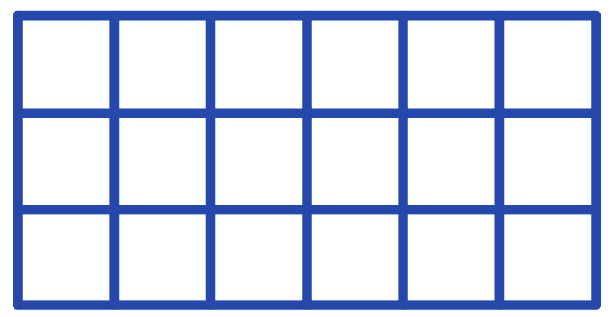
\includegraphics[scale=0.35]{tab.png}}
\end{figure}\\
Расставьте в каждую клетку таблицы $3\times6$ букву М, Я или П так, чтобы у каждой М было 4 соседа Я, а у каждой П было ровно два соседа Я, а у каждой Я среди соседей есть и М, и П. Соседи считаются только по стороне.\\
